\section{Equivalence of RTL and Software Netlist}
%
The consistency between two designs can be established in several ways. 
For example, a few common notions of consistency are \emph{behavioral}, 
\emph{cycle-accurate}, \emph{non-cycle accurate} or \emph{functional}
consistency.  The consistency between a reference model and an implementation
model is established through systematic equivalence 
checking~\cite{CKY03,DBLP:conf/date/KoelblJJP09,DBLP:journals/tcad/StoffelK04,
DBLP:conf/date/Eijk98,DBLP:conf/iccd/BaumgartnerMPKJ06}.  Equivalence checking between a timed and untimed model is a hard
problem~\cite{kuehlmann2002combinational}.  Sequential equivalence checking techniques 
are used to check the equivalence between an asynchronous event driven semantics of C and synchronous 
clock driven semantics of Verilog~\cite{CKY03, DBLP:conf/iccd/BaumgartnerMPKJ06}.


%%%%%%%%%%%%%%%%%% CYCLE ACCURATE EQUIVALENCE %%%%%%%%%%%%%%%%%
Two designs are said to be \emph{cycle-accurate-equivalent}~\cite{cycle,kuehlmann2002combinational} 
if they produce the same output using the same number of clock cycles.   
%%%%%%%%%%%%%%%%%% NON-CYCLE ACCURATE EQUIVALENCE %%%%%%%%%%%%%%%%%
Whereas, two designs are \emph{not} cycle-accurate-equivalent if they require 
different cycles to perform the same computation. For example, consider two circuits
implementing Euclid's algorithm to compute Greatest Common Divisor (GCD),
where Circuit A uses two subtractors and Circuit B uses one subtractor. Assume that 
Circuit B requires more cycle than Circuit A for computing the GCD. Thus,
they are functional-equivalent but not cycle-accurate-equivalent. However,
Circuit A and Circuit B can be made cycle-accurate-equivalent by making Circuit
A to stutter for few cycles until Circuit B finishes its slower operation.  This
may require some additional logic in Circuit A to determine the condition for 
stuttering.  


In this paper, we consider an equivalence between RTL and software netlist 
that preserves both the input-output behavior and the validity of all assertions 
(temporal or non-temporal) originating in the RTL in the software netlist.  
We describe this next.
% 
%%%%%%%%%%%%%%%%%% LTL Semantics to C %%%%%%%%%%%%%%%%%
\para{Properties}~\label{prop}
%
System Verilog Assertions (SVA) property specification language is most commonly used 
to write properties of RTL designs.  The SVA properties can be translated 
into an intemediate Linear Temporal Logic (LTL)~\cite{DBLP:journals/jacm/SistlaC85} 
representation.  LTL is a modal logic that is commonly used to reason about a hardware 
transition system.  The modalities in LTL refers to
temporal operators such as $G$ (global), $F$ (eventual), $X$ (next) and $U$
(until).  An LTL formula may contain propositional symbols, boolean or temporal
operators.  We refer the reader to~\cite{DBLP:journals/jacm/SistlaC85,mc-book} 
for more details on LTL. 


The translation of LTL to a \emph{Buchi Automaton}
(BA) is a well-known technique~\cite{Gastin:2001, SomenziB00} and has been
successfully used for LTL model checking, such as the Spin model checker~\cite{spin}.   
Further, a Buchi Automaton can be modeled using a C program that simply encodes
its state transition relation.  
%
In this work, we use System Verilog Assertions (SVA) to express properties of 
the RTL designs. The SVA properties are translated into equivalent C assertions 
either using \emph{v2c} or manually.
%
\Omit{
The translation of purely propositional properties is straightforward.  While, 
the translation of temporal properties are done following the notion of equivalence 
described in Section~\ref{eq-sw-hw}. 
}
%


Figure~\ref{prop} gives an example of SVA, its equivalent LTL, 
and the corresponding assertion in the software netlist for the 
design of Figure~\ref{figure:equivalence}.
%
The next time operator $X$ in LTL is 
modeled by invoking the top-level procedure
$M(clk,in,out1,out2,out3)$ in the software netlist. 
Note that the top-level procedure in the software netlist 
corresponds to the top-level module of the RTL design.  
%
\Omit{
The granularity 
of the effect of one clock step is modeled by invoking 
the top-level procedure in the software netlist.
}
%
\begin{figure}[t]
\scriptsize  
\centering
\begin{tabular}{|l|l|}
\hline
 Buchi Automaton & Assertion in $\mathcal{SN}$ \\
\hline
\begin{minipage}{3.5cm}
\scalebox{.5}{\import{figures/}{property.pspdftex}}
\end{minipage}
&
\begin{lstlisting}[mathescape=true,language=C]
if(sM.out2) {
  M(clk,in,out1,out2,out3);
  assert(sM.out3);
}
\end{lstlisting}
\\
\hline
\end{tabular}
\caption{LTL and its corresponding C assertion}
\label{prop}
\end{figure}
%
%The goal of this translation is to perform formal property verification 
%of the software netlist against the assertions given in SVA.
%expressed over the variables of $\mathcal{SN}$.  
%
%%%%%%%%%%%%%%%%%% RESTRICTED CYCLE ACCURATE EQUIVALENCE %%%%%%%%%%%%%%%%%
\para{Property-based Observable Equivalence}
%
Recall that a RTL design in Verilog is translated into a software 
netlist in C for the purposes of formal verification.  To this end, the formal specification or 
properties (temporal or non-temporal) over RTL signals that captures hardware behaviors 
are translated into assertions over the corresponding software variables in 
the software netlist and checked for consistency against the software
netlist.  Thus, our notion of equivalence is based on the signals 
that are observable in the properties under consideration.  We call this equivalence criteria 
\emph{property-based observable equivalence}.  
Intuitively, this means that the state of latches and wires 
referred to by the property must match with the corresponding variables in the 
software netlist at some designated clock cycle.  Recall that the effect of a clock cycle 
in the software netlist is simulated through an invocation of the top 
level procedure which corresponds to the top level module of the RTL~\cite{mtk2016}.  
By means of experiment, we show that the proposed notion of equivalence is sufficient for the 
purposes of property-based verification.
%
\Omit{Note that a software netlist is synthesized from a hardware
RTL for the purposes of formal verification, just like a bit-level netlist or
word-level netlist are synthesized from an RTL. So, the proposed consistency 
criteria is sufficient for this purpose.}  
%
\begin{definition}~\label{verilog-c-eq} (Property-based Observable Equivalent) 
  Two designs $C_1$ and $C_2$ are \emph{property-based observable equivalent} with
  respect to a property $P$ if the following conditions hold.  Note that we assume 
  that the verification outcome of these properties are obtained using the native 
  verifiers for software and hardware.  The verification outcome can be 
  either \emph{safe} in which case $P$ holds on $C_1$ and $C_2$, or \emph{unsafe} 
  in which case $P$ does not hold on $C_1$ and $C_2$. 
  \begin{enumerate}
    \item For a non-temporal property $P$, the verification outcome of $P$ must
      match in $C1$ and $C2$ at every clock cycle.  
   \item For a temporal property $P$, the verification outcome of $P$ must 
     match in $C_1$ and $C_2$ at some \emph{designated} clock cycle.  Such
      designated clock cycle is determined by the temporal operator used in $P$. 
  \end{enumerate}
\end{definition}
%
Two designs $C_1$ and $C_2$ are \emph{not} property-based observable equivalent 
with respect to a non-temporal property $P$ if there exist a clock cycle where 
the verification outcomes of $P$ in $C_1$ and $C_2$ do not match.  Intuitively, 
this means that at some cycle $N$, 
%there exists some latches or wires 
the state of latches or wires that are referred to by $P$, does not match in 
$C_1$ and $C_2$, resulting in inconsistent verification outcome for $P$. 
% 
Whereas, two designs $C_1$ and $C_2$ are \emph{not} property-based observable equivalent 
with respect to a temporal property $P$ if there exists a \emph{designated} clock cycle 
where the verification outcomes of $P$ in $C_1$ and $C_2$ do not match.  



%%%%%%%%%%%%%%%%%% EXAMPLE %%%%%%%%%%%%%%%%%
\begin{example}
%
Figure~\ref{figure:equivalence} gives an example of a Verilog RTL design 
(on the left) and the corresponding software netlist in C (on the right) that are 
property-based observable equivalent with respect to a temporal 
property (marked in blue).  The property in the Verilog RTL design 
is specified in SystemVerilog Assertion (SVA)~\cite{SVA} language.  
The equivalent assertion in the software netlist is shown on the right (marked in blue).  


Figure~\ref{fig:waveform} gives the waveform view of 
the operation of the design. 
%
We explain the equivalance of the Verilog RTL and the 
software netlist design with respect to the temporal SVA 
assertion, \texttt{assert property(in==1 |-> \#\#1 out3)}.  
%


Suppose $in=1$ at clock cycle $i$.  Then, the state of 
the latch $out3$ is not consistent in Verilog and C at 
cycle $i$.  This is due to the fact that 
the value of $out3$ \emph{stabilizes} one cycle after the 
input $in=1$ was set, that is, $out3$ is stabilized in cycle $i+1$.  
This behavior is formally captured 
in SVA by the expression \texttt{(in==1 |-> \#\#1 out3)}.  
The SVA property specifies that the latch $out3$ is high 
exactly one cycle after $in$ was high.  
%

Recall from Definition~\ref{verilog-c-eq} that for two designs to be property-based 
observable equivalent with respect to a temporal property $P$,  the 
verification outcome of $P$ must match in the two designs at some 
designated clock cycle. 
%
In this case, the designated clock cycle is specified by \texttt{\#\#1}
delay operator.  That is, the value of $out3$ must match in Verilog 
and the software netlist one cycle after the event $in==1$ has occured. 
%
Thus, the value of $out3$ may be inconsistent in Verilog and software netlist 
in the same cycle when $in==1$, but the property still holds in both the designs. 
%
We use a state-of-the-art hardware model checker and a commercial 
software analyzer to verify the RTL and the software netlist respectively.  
The property is proven equivalent for unbounded cycles in Verilog RTL 
and the software netlist design.
%
Hence, both the designs are property-based observable equivalent. 
\end{example}
%
%
\begin{figure}[t]
\centering
\scriptsize
\begin{tabular}{l|l}
\hline
Verilog RTL & Software netlist (in C) \\
\hline
\begin{lstlisting}[mathescape=true,language=Verilog,style=base]
module M(clk, in, 
     out1, out2, out3);
input clk,in;
output reg out1, 
     out2, out3;
wire t1;

initial begin
out1=0; 
out2=0;out3=0;
end

assign t1=out1;

always @(in) begin
out1 <= in;
end

always@(t1) begin
out2 <= t1;
end

always@(posedge clk) 
begin
out3 <= out2;
end
endmodule

module main(clk);
input clk;
wire in,out1,
     out2,out3;
M m1(clk,in,out1,out2,out3);
~assert property ~
 ~(in |-> ##1 out3);~
endmodule
\end{lstlisting}
&
\begin{lstlisting}[mathescape=true,language=C,style=base]
struct state_M {
 bool out1, out2, out3; 
};
struct state_M sM;

void initial() {
 sM.out1=0; sM.out2=0; 
 sM.out3=0;
}

void M(bool clk, bool in, 
 bool *out1, bool *out2, 
 bool *out3) {
  bool t1;
  sM.out1=in;
  t1=sM.out1;
  sM.out2=t1;
  sM.out3=sM.out2;
  // update output  
  *out1=sM.out1;
  *out2=sM.out3;
  *out3=sM.out3;
}
 
int main()
{
 bool clk,in,
 out1,out2,out3;
 initial();
 ~while(1) {~
  ~if(in) {~
   ~M(clk,in,~
   ~&out1,&out2,&out3);~
   ~assert(sM.out3);~
  ~}~
 ~}~
}
\end{lstlisting}
\\
\hline
\end{tabular}
\caption{Property-based observable equivalence}
\label{figure:equivalence}
\end{figure}
%
\begin{figure}[t]
\begin{center}
  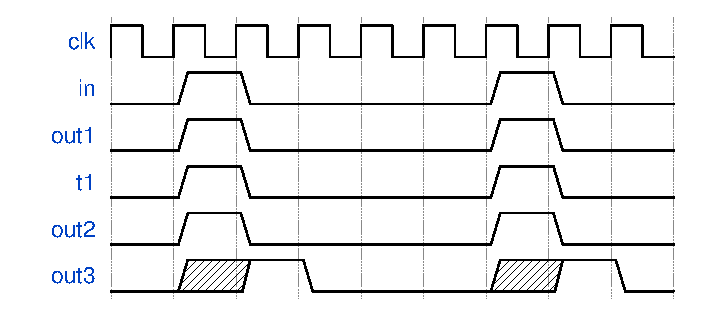
\includegraphics[width=\columnwidth]{figures/wavedrom.eps}%
  \caption{Waveform view showing behavior of RTL design in
  Figure~\ref{figure:equivalence}} 
\label{fig:waveform}
\end{center}
\end{figure}
%
Techniques such as translation validation~\cite{DBLP:conf/tacas/PnueliSS98}  
that check the consistency between an RTL and software is a different problem 
and beyond the scope of this work.
%
%While we do not have a formal proof of equivalence between the Verilog RTL and the 
However, experiments have shown that for 
property verification, valid safety properties are proven to be $k$-inductive for 
the same unwind depth $k$ in the RTL and the software netlist design.  Conversely, 
for unsafe designs, a bug is found in the same unwind depth for both the designs.

